
\begin{figure}[H]
\newcommand{\wmgd}{1\columnwidth}
\newcommand{\hmgd}{3.0cm}
\newcommand{\mdrd}{figures/mean-monthly-air-temperature-deg}
\newcommand{\mbm}{\hspace{-0.3cm}}
\begin{tabular}{c}
\mbm 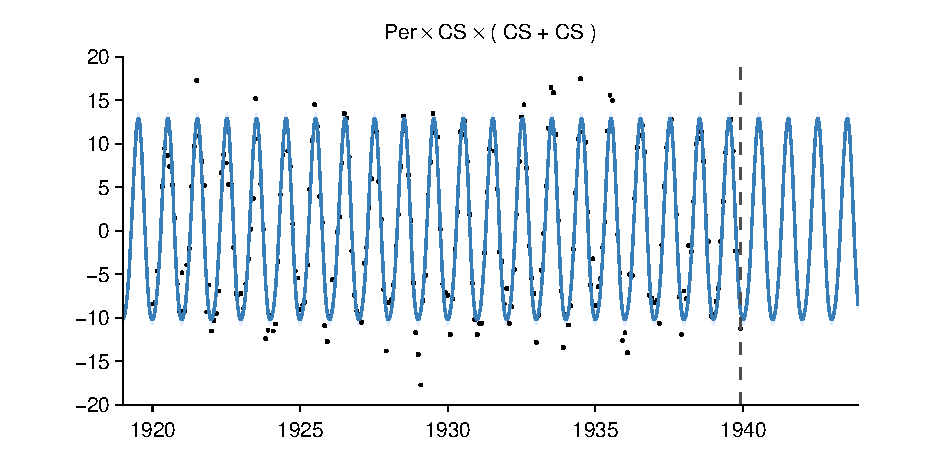
\includegraphics[width=\wmgd,height=\hmgd]{\mdrd/mean-monthly-air-temperature-deg_all} \\ = \\

\mbm 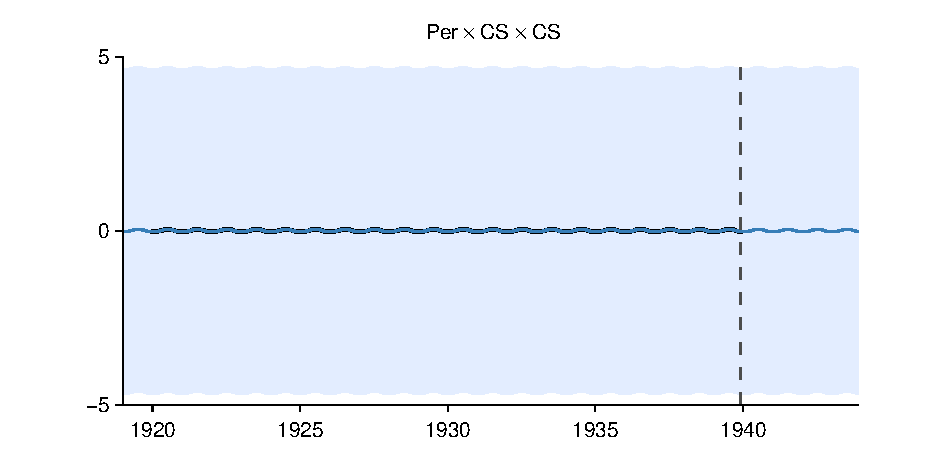
\includegraphics[width=\wmgd,height=\hmgd]{\mdrd/mean-monthly-air-temperature-deg_1} \\ + \\

\mbm 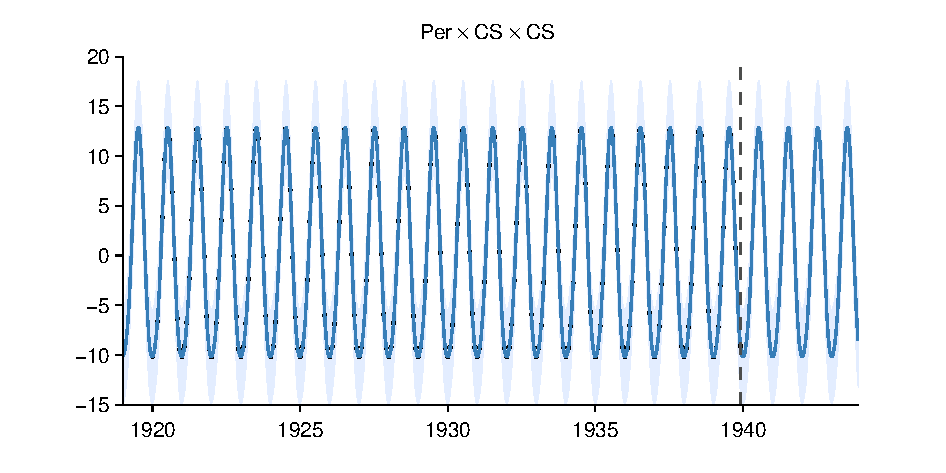
\includegraphics[width=\wmgd,height=\hmgd]{\mdrd/mean-monthly-air-temperature-deg_2} \\ + \\

\mbm 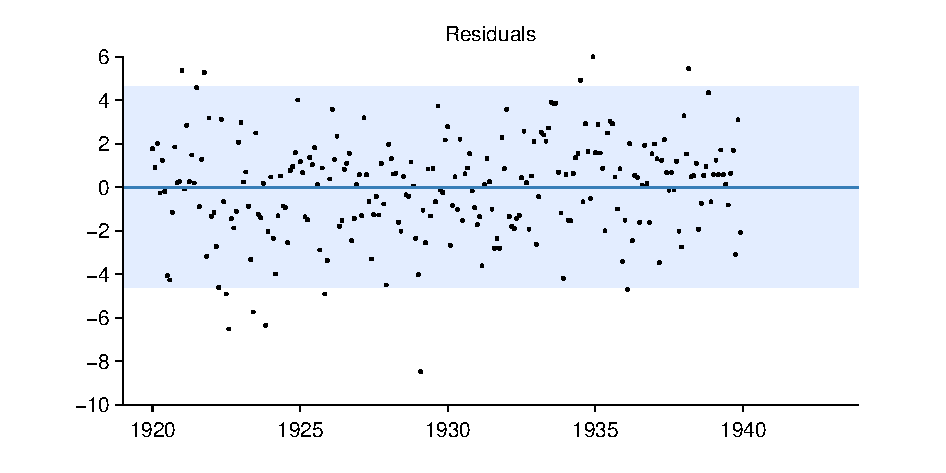
\includegraphics[width=\wmgd,height=\hmgd]{\mdrd/mean-monthly-air-temperature-deg_resid}
\end{tabular}
\end{figure}
